\textbf{The infamous Runge-Phenomenon:} It is not generally true that higher degree interpolation polynomials yield more accurate approximations. This is illustrated in this problem. Let \[f(x) = \frac{1}{1+x^2}\text{    and    }x_j = -5 + jh\text{,    }j=0,1,\dots,n\text{,    }h = \frac{10}{n}.\] For \[n=1,2,3,\dots,20\] plot the graph (in the interval $[-5,5]$) of the interpolant \[p(x) = \sum_{i=0}^n \alpha_i x^i\] defined by \[p(x_i) = f(x_i)\text{,    }i=0,1,\dots,n.\]

{\color{blue}

\begin{figure}[H]
\centering
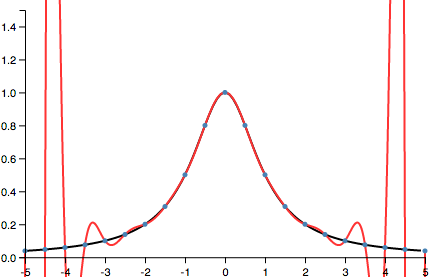
\includegraphics[scale=0.65]{runge-equidistant.png}
\caption{We interpolate points obtained from the Runge function across
  an equidistant interval with $n=20$ in red. The original Runge
  function is plotted in black, along with the points we've
  interpolated from. The interpolated polynomial fluctuates wildly at
  either end of our domain.}
\end{figure}

\begin{figure}[H]
\centering
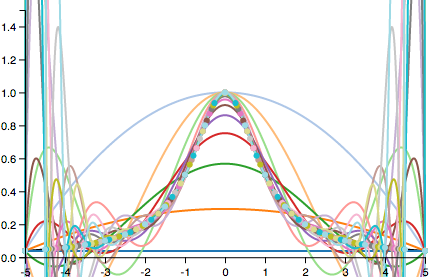
\includegraphics[scale=0.65]{runge-equidistant-n-1-20.png}
\caption{Interpolating several functions for $n = 1,\dots,20$}
\end{figure}

We can see that as we interpolate more points the center of our
function gets approximated better, but the end points become more
unstable. They fluctuate greatly trying to interpolate all points on
the interval.

}
